\documentclass[conference]{IEEEtran}
\usepackage[T1]{fontenc}
\usepackage{graphicx}
\usepackage{booktabs}
\usepackage{amsmath}
\usepackage{amssymb}
\usepackage{algorithm}
\usepackage{algpseudocode}
\usepackage{array}
\usepackage{tabularx}
\usepackage{url}
\usepackage{cite}
\usepackage[hidelinks]{hyperref}

% Every number in this file comes from claims.md (and the files it names). Change a
% number there first, then here.

% Anonymous build for double-blind review: define \anonymous before loading the file,
% e.g. latexmk -pdf -jobname=paper-anon -usepretex='\def\anonymous{}' paper.tex
\newif\ifanon
\ifdefined\anonymous\anontrue\fi

\begin{document}

\title{An Empirical Evaluation of Static Analysis Finding Identity Across Code
Changes}

\ifanon
\author{\IEEEauthorblockN{Anonymous Author(s)}}
\else
% TODO(author): add the affiliation line before submission.
\author{\IEEEauthorblockN{Vichitra Attri}
\IEEEauthorblockA{mevichitra@gmail.com}}
\fi

\maketitle

\begin{abstract}
Baselines, suppressions, alert de-duplication and CI gates that fail only on new
findings all depend on a
static analysis tool recognizing a finding it reported on the previous commit. We
measure how well the methods that shipped tools use for this work. We ported
SonarQube's issue tracker, Bandit's baseline comparison, Semgrep's match ID and the line
hash that GitHub's CodeQL Action uploads as a fingerprint, checked each port against the original, and
replayed 200 consecutive commit pairs from each of 35 open-source web
applications, with findings from three analyzers, scoring every method against a line-diff ground truth that also detects
moved code. Line numbers report
52.6\% of persisting findings as new; the other methods report 0.4--4.4\%. Much of what
remains comes from renamed files. They hold 1.2\% of persisting findings, and every
method whose identity includes the path reports all of them as new; SonarQube loses
2.8\% of them in pull-request analyses and 20.2\% in branch analyses. Bandit's baseline
matches by set membership: it hides 27.3\% of Bandit's own new findings, and a CI gate
built on it stays silent on 34.1\% of the commit pairs that introduce one, where every
other method misses none. Semgrep's own ID, which numbers equal matches in file order,
hides 12.1\% of Semgrep's new findings. Ten controlled code transformations show that each method has
a change it cannot follow.
\end{abstract}

\section{Introduction}

A static analysis tool that runs on every commit has to decide, for each finding,
whether it reported that finding before. Baselines rest on this decision, and so do
suppressions, alert de-duplication and CI gates that fail only on new findings. It can
go wrong in two ways. An old finding reported as new is noise: the baseline breaks, and
developers are asked again about code they did not touch. A new finding taken for an
old one is \emph{hidden}. For a security gate that is the expensive error, since the
vulnerability passes the check that was meant to stop it.

Tools answer the question in very different ways (Section~\ref{sec:schemes}), mostly
documented only in their source code, and we know of no study that measures them against one
another on the same findings: earlier work built a better tracker for one family of
tools~\cite{li2022statictracker} or used a tracker as a step in studying
developers~\cite{avgustinov2015,kim2007}.

We ask two questions. \textbf{RQ1:} over real commit histories, how often does each
tool's method report a persisting finding as new, and how often does it hide a new one?
\textbf{RQ2:} which kinds of code change break which methods?

To answer them we replay commit histories and score each method against an independent
ground truth, a line diff that also detects moved code, which a manual check of 100
findings supports (Section~\ref{sec:threats}). This paper contributes:
\begin{itemize}
\item ports of the identity methods of SonarQube, Bandit and Semgrep, and of the
  fingerprint the CodeQL Action computes for GitHub code scanning, each checked against
  the original code;
\item RQ1 on 7,000 commit pairs from 35 open-source web applications, with findings from
  three analyzers, and RQ2 on ten controlled transformations;
\item two results that tool builders can act on: putting the file path into a
  finding's identity causes most of the false-new reports of \texttt{codeguard} and
  \texttt{line\_text}, and matching by set membership hides new findings, so that a
  gate built on it misses a third of the commits that add a Bandit finding;
\item the replay tool, the corpus, the results and the scripts behind every number,
  under Apache-2.0.
\end{itemize}

\section{Identity Schemes}\label{sec:schemes}

A \emph{scheme} decides which finding in the new version of a file, if any, is the same
as a given finding in the old version. Findings are compared only within one rule. Four
schemes build a key and pair findings with equal keys, one to one, in line order; the
other three run a matching algorithm (Table~\ref{tab:schemes}). \texttt{codeguard} is the
fingerprint of CodeGuard, \ifanon the authors' own open-source analyzer\else the
open-source analyzer the author maintains\fi. \texttt{github} is the
\texttt{primaryLocationLineHash} that the CodeQL Action uploads in SARIF's
\texttt{partialFingerprints}; we pair by that key alone, so we measure the fingerprint,
not how GitHub's service matches results to open alerts.

SonarQube's tracker tries six passes in turn: rule, line, line hash and message; rule,
line and line hash; code moves, by unique 11-line block hashes and then the longest
identical block; rule, line hash and message; rule, line and message; rule and line
hash. The line hash is the MD5 of the line without spaces and tabs. A pull-request
analysis (\texttt{sonar}) takes renames from the SCM; a branch analysis
(\texttt{sonar\_branch}) keeps a renamed file's findings only if its own file move
detection accepts the rename. With $n$ and $n'$ the old and new line counts and $h$ and
$h'$ the files' sequences of line hashes, it requires
\begin{equation}\label{eq:move}
\lfloor 0.84\,n \rfloor < n' < \lceil 1.18\,n \rceil
\ \ \text{and}\ \
\Bigl\lfloor 100 \Bigl(1 - \frac{d(h, h')}{\max(n, n')}\Bigr) \Bigr\rfloor \ge 85,
\end{equation}
where $d$ is the Levenshtein distance between the two sequences, each line counting as
one symbol.

\begin{table}[t]
\centering
\caption{The identity schemes compared. Path: whether the file path is part of the
identity, so that findings in a renamed file cannot match; checked: a rename
counts only if SonarQube's file move detection accepts it.}
\label{tab:schemes}
\footnotesize
\setlength{\tabcolsep}{3pt}
\begin{tabularx}{\columnwidth}{@{}l>{\raggedright\arraybackslash}Xll@{}}
\toprule
Scheme & Identity built from & Pairing & Path \\
\midrule
\texttt{line} & line number & key & yes \\
\texttt{line\_text} & exact text of the flagged line & key & yes \\
\texttt{github} & the CodeQL Action's \texttt{primaryLocationLineHash}: a rolling hash over the
  100 non-blank characters from the start of the line, plus an occurrence index & key &
  yes \\
\texttt{codeguard} & enclosing function or class, plus the statement with literals
  masked and comments and whitespace removed & key & yes \\
\texttt{sonar} & SonarQube's tracker, pull-request analysis & 6 passes & no \\
\texttt{sonar\_branch} & SonarQube's tracker, branch analysis & 6 passes & checked \\
\texttt{bandit} & \texttt{bandit -b}: issue text, severity, confidence, CWE, file and
  test; no location & set & yes \\
\bottomrule
\end{tabularx}
\end{table}

Bandit's baseline does not pair findings: a result is known when an equal issue is in
the baseline, so one baselined issue hides any number of equal new ones.

\section{Method}\label{sec:method}

\textit{Ground truth.} Let $O$ and $N$ be the findings in the old and the new version of
a file that a commit changes; a finding $f$ has a rule $r(f)$, a line $\ell(f)$ and a
column $c(f)$. Renamed files are paired by \texttt{git diff -M}. A line diff (Python's
\texttt{difflib}) splits the two versions into unchanged and replaced blocks and yields
a partial map $\mu$ from old lines to new ones. Unchanged lines map one to one. Inside a
replaced block with old lines $a_1, \dots, a_p$ and new lines $b_1, \dots, b_q$, two
lines, stripped of surrounding whitespace, are compared by
\begin{equation}\label{eq:sim}
s(a, b) = \frac{2M}{|a| + |b|},
\end{equation}
where $M$ is the number of characters in the matching blocks that Ratcliff and
Obershelp's algorithm finds (difflib's \texttt{ratio}). The lines of the block are then
paired in order so that their total similarity is largest, counting only pairs with
$s \ge \theta = 0.6$:
\begin{equation}\label{eq:align}
B_{i,j} = \max \bigl( B_{i+1,j},\ B_{i,j+1},\ s(a_i, b_j) + B_{i+1,j+1} \bigr),
\end{equation}
where the third term applies only when $s(a_i, b_j) \ge \theta$, and
$B_{p+1,j} = B_{i,q+1} = 0$. Tracing back from $B_{1,1}$ gives the pairs. A block with
$pq > 40{,}000$ is aligned only in a band around its diagonal, which bounds the cost; no
finding in our replays fell in such a block.

Lines still unmapped can be moved code. Following Git's moved-line detection
(\texttt{git diff --color-moved}), a run of consecutive unmapped old lines that
reappears line for line, ignoring surrounding whitespace, as consecutive unmapped new
lines is mapped as \emph{relocated} when it holds at least 20 alphanumeric characters and
its text occurs exactly once in each version, so the map never guesses between copies.
Blocks are taken greedily, largest first. Where two moved blocks are separated by at most
10 unmapped lines on each side, those lines are aligned by \eqref{eq:align}; an edit at
either end of a moved block is lost, and moves between files are not detected. Nothing
here reuses SonarQube's block hashes. Deleted lines, and lines replaced past the
threshold, stay unmapped.

The ground truth $T\colon N \rightharpoonup O$ pairs the findings. Taking old findings in
order of line and column, it pairs each $o$ with the still unpaired $n \in N$ that has
$r(n) = r(o)$ and $\ell(n) = \mu(\ell(o))$, choosing the column nearest $c(o)$. The
\emph{persisting} findings are $K = \operatorname{dom} T$, the \emph{introduced} ones
$I = N \setminus K$. No scheme takes part in this.

\textit{Outcomes and metrics.} A scheme $\sigma$ gives its own partial pairing
$P_\sigma\colon N \rightharpoonup O$. The four key schemes group the findings by key,
sort each group by line and column in both versions, and pair the $i$-th old finding with
the $i$-th new one. SonarQube and Bandit run their ported matchers, and
\texttt{sonar\_branch} pairs nothing across a rename that \eqref{eq:move} rejects. A
persisting finding $n$ is \emph{known} if $P_\sigma(n) = T(n)$, \emph{mispaired} if
$P_\sigma(n)$ is another old finding and \emph{false new} if $P_\sigma(n)$ is undefined;
an introduced finding is \emph{hidden} if $P_\sigma(n)$ is defined. Summed over all file
pairs of a replay, the two main rates are
\begin{equation}\label{eq:rates}
\mathrm{FN}_\sigma = \frac{|K \setminus \operatorname{dom} P_\sigma|}{|K|},
\qquad
\mathrm{H}_\sigma = \frac{|I \cap \operatorname{dom} P_\sigma|}{|I|}.
\end{equation}
The \emph{collision rate} $\mathrm{C}_\sigma$ is the share of findings, over every file
version the replay analyses, that share their $\sigma$ key with another finding in the
same version; for those findings the pairing falls back on line order. The key of
\texttt{sonar} is rule, path and line hash (that of its last pass), and that of
\texttt{bandit} is the tuple Bandit compares: issue text, severity, CWE, confidence,
file and test. Algorithm~\ref{alg:replay} puts the steps together; it skips files the
analyzer does not read (vendored, generated and minified code).

\textit{The gate.} A CI gate that fails on new findings sees one commit pair at a time.
With $N_t$ the findings in the changed files of pair $t$ and $I_t \subseteq N_t$ the
introduced ones, the gate fires when $G_\sigma(t)$ holds and should fire when $G^*(t)$
does:
\begin{equation}\label{eq:gate}
G_\sigma(t) = \bigl[\, \exists\, n \in N_t : n \notin \operatorname{dom} P_\sigma \,\bigr],
\qquad
G^{*}(t) = \bigl[\, I_t \neq \emptyset \,\bigr].
\end{equation}
With $T^{+}$ the pairs where $G^{*}$ holds and $T^{-}$ the others, the miss and
false-alarm rates are
\begin{equation}\label{eq:gaterates}
\mathrm{Miss}_\sigma = \frac{|\{t \in T^{+} : \neg G_\sigma(t)\}|}{|T^{+}|},
\
\mathrm{FA}_\sigma = \frac{|\{t \in T^{-} : G_\sigma(t)\}|}{|T^{-}|}.
\end{equation}
A hidden finding is \emph{masked} when its pair's gate fires anyway, because the scheme
reports another finding of the pair as new, and \emph{silent} otherwise; the two add up
to the hidden rate.

\begin{algorithm}[t]
\caption{Replaying and scoring one repository}\label{alg:replay}
\small
\algrenewcommand\algorithmicindent{1em}
\begin{algorithmic}[1]
\Require a repository and branch, $k = 200$, schemes $\Sigma$
\State $c_0, \dots, c_k \gets$ the last $k+1$ first-parent commits, oldest first
\For{$t = 1, \dots, k$}
  \ForAll{changed file $(p, p')$ from $c_{t-1}$ to $c_t$}
    \State $O, N \gets$ findings in $p$ at $c_{t-1}$, in $p'$ at $c_t$
      \Comment{$\emptyset$ if absent}
    \State $\mu \gets$ line map by \eqref{eq:sim}, \eqref{eq:align} and moved blocks
    \State $T \gets \textsc{GroundTruth}(O, N, \mu)$
    \ForAll{$\sigma \in \Sigma$}
      \State $P \gets \textsc{Pair}_\sigma(O, N)$
      \State \textbf{if} $\sigma = \texttt{sonar\_branch}$, $p \ne p'$ and
        \eqref{eq:move} rejects the rename: $P \gets \emptyset$
      \ForAll{$n \in N$}
        \State count the outcome of $n$ for $\sigma$ from $T(n)$ and $P(n)$
      \EndFor
    \EndFor
  \EndFor
\EndFor
\State \Return the counts per scheme and outcome
\end{algorithmic}
\end{algorithm}

\textit{Corpus.} We chose 35 open-source web applications by written criteria:
deployable applications with at least 100 analysable back-end files that handle user
requests, at least 200 first-parent commits in the two years before the pin, one
OSI-approved licence and no committed build output. Twenty-five are Python projects (16 Django, 4 Flask, 2 FastAPI, and one each on
Pyramid, web.py and Frappe), ten JavaScript or TypeScript (5 Express, 3 NestJS,
2 Next.js). Each was pinned on 2026-10-14, and we replayed its last 200 first-parent
commit pairs.

\textit{Findings.} CodeGuard 2.2.0 analysed all 35 repositories: 23,245 persisting and
1,966 introduced findings over 7,000 commit pairs. Bandit 1.9.4 analysed the 25 Python
repositories (5,000 pairs), without B101, which flags every \texttt{assert} and would
dominate the hidden rate with its constant message: it is 91.0\% of Bandit's persisting
findings, 98\% of them in test code. That leaves 15,746 persisting and 1,069 introduced
findings. A third set comes from rules that nobody involved in this study wrote: Semgrep
1.180.0 ran the 587 Python, JavaScript and TypeScript rules of the opengrep-rules fork of
semgrep-rules (commit \texttt{f1d2b56}, LGPL-2.1 with the Commons Clause) on all 35
repositories, for 57,166 persisting and 4,328 introduced findings.

\textit{Ports and their checks.} The SonarQube port follows SonarQube 26.10.0.133078; on
20,000 generated cases it agrees with the unmodified Java tracker, compiled from the
same tag, every time. The Bandit port flags exactly the issues a live
\texttt{bandit -b} run reports, including a hidden duplicate. The GitHub port reproduces
the hashes that the CodeQL Action's own \texttt{fingerprints.ts} computes on reference inputs with
duplicate, blank, CRLF and CR-only lines. Over the Semgrep run, the port
reproduced 87,916 of the 87,924 \texttt{match\_based\_id} values Semgrep emitted. The
other 8 were two taint results at one sink, which Semgrep numbers in source order but
reports in message order; the port now does the same.

\textit{Statistics.} Every rate is pooled over repositories: with $x_r$ and $y_r$ the
numerator and denominator of \eqref{eq:rates} in repository $r$,
$R = \sum_r x_r / \sum_r y_r$. Findings within a repository are correlated, so the 95\%
interval comes from a cluster bootstrap. Each of $10{,}000$ resamples draws as many
repositories as the corpus has, with replacement; the interval runs from the 2.5th to
the 97.5th percentile of the resampled $R^{(b)}$. A resample with a zero
denominator is dropped, and every table uses the same draws, so differences between
schemes get paired intervals. The renamed-file column rests on the 8 repositories with
renames; no resample of CodeGuard findings lacked all of them. A per-finding interval
would be far too narrow: for \texttt{line\_text}'s false-new rate of 1.91\%, the Wilson
interval is 1.75--2.10 and the cluster bootstrap gives 0.81--3.54.

\textit{RQ2 transformations.} We used ten transformations, each applied with libcst to one
target finding in each of 40 sampled files per Python repository (Fig.~\ref{fig:rq2}).
\texttt{reformat} runs black at 79 columns; \texttt{insert\_top} adds a comment and an
unused import at the top of the module; \texttt{move\_function} swaps the enclosing
function with its neighbour; \texttt{extract\_helper} moves the statement into a new
function; the two \texttt{duplicate} edits copy the statement and so introduce a
finding. Each transformation returns an exact old-to-new line map, the ground truth by
construction, and skips files it does not fit, leaving 150 (\texttt{extract\_helper}) to
937 (\texttt{insert\_top}) cases each.

\section{RQ1: Real Histories}\label{sec:rq1}

% Generated by research/finding_identity/paper_kit.py; do not edit by hand.
\begin{table*}[t]
\centering
\caption{Identity errors over 200 consecutive commit pairs per repository, in percent: pooled rate with its 95\% cluster-bootstrap interval over repositories. CodeGuard findings: 35 repositories, 23,245 persisting and 1,966 introduced findings, 287 of the persisting ones in renamed files. Bandit findings other than B101: 25 Python repositories, 15,746 persisting and 1,069 introduced findings.}
\label{tab:rq1}
\setlength{\tabcolsep}{3pt}
\begin{tabular}{lrrrrrrrr}
\toprule
 & \multicolumn{6}{c}{CodeGuard findings} & \multicolumn{2}{c}{Bandit findings} \\
\cmidrule(lr){2-7} \cmidrule(lr){8-9}
 & \multicolumn{3}{c}{False new} & Mispaired & Hidden & Collisions & False new & Hidden \\
\cmidrule(lr){2-4}
Scheme & all & same path & renamed \\
\midrule
\texttt{line} & 52.6 {\scriptsize(48.5--57.6)} & 52.0 {\scriptsize(48.1--56.8)} & 100.0 {\scriptsize(100.0--100.0)} & 2.8 {\scriptsize(1.6--3.9)} & 1.2 {\scriptsize(0.6--2.2)} & 2.1 {\scriptsize(1.1--3.5)} & 55.0 {\scriptsize(49.6--61.7)} & 2.0 {\scriptsize(0.4--4.2)} \\
\texttt{line\_text} & 1.9 {\scriptsize(0.8--3.5)} & 0.7 {\scriptsize(0.5--0.9)} & 100.0 {\scriptsize(100.0--100.0)} & 0.2 {\scriptsize(0.1--0.4)} & 1.0 {\scriptsize(0.5--1.9)} & 17.4 {\scriptsize(14.0--21.3)} & 0.9 {\scriptsize(0.6--1.3)} & 5.2 {\scriptsize(2.2--9.0)} \\
\texttt{github} & 3.1 {\scriptsize(2.0--4.9)} & 1.9 {\scriptsize(1.6--2.3)} & 100.0 {\scriptsize(100.0--100.0)} & 0.1 {\scriptsize(0.0--0.2)} & 0.5 {\scriptsize(0.1--1.2)} & 2.1 {\scriptsize(1.1--3.5)} & 2.0 {\scriptsize(1.1--3.2)} & 2.0 {\scriptsize(0.7--3.5)} \\
\texttt{codeguard} & 1.8 {\scriptsize(0.7--3.4)} & 0.6 {\scriptsize(0.4--0.8)} & 100.0 {\scriptsize(100.0--100.0)} & 0.3 {\scriptsize(0.1--0.7)} & 1.5 {\scriptsize(0.8--2.8)} & 18.6 {\scriptsize(12.9--24.8)} & 0.5 {\scriptsize(0.2--0.8)} & 0.7 {\scriptsize(0.1--1.6)} \\
\texttt{sonar} & 0.4 {\scriptsize(0.3--0.6)} & 0.4 {\scriptsize(0.2--0.5)} & 2.8 {\scriptsize(1.7--8.3)} & 0.2 {\scriptsize(0.1--0.3)} & 1.1 {\scriptsize(0.7--1.9)} & 20.3 {\scriptsize(16.5--24.4)} & 0.3 {\scriptsize(0.1--0.5)} & 2.0 {\scriptsize(0.2--4.6)} \\
\texttt{sonar\_branch} & 0.6 {\scriptsize(0.3--1.0)} & 0.4 {\scriptsize(0.2--0.5)} & 20.2 {\scriptsize(4.3--62.3)} & 0.2 {\scriptsize(0.1--0.3)} & 1.1 {\scriptsize(0.6--1.8)} & 20.3 {\scriptsize(16.5--24.4)} & 0.3 {\scriptsize(0.1--0.5)} & 2.0 {\scriptsize(0.2--4.6)} \\
\texttt{bandit} & 4.4 {\scriptsize(3.1--6.3)} & 3.2 {\scriptsize(2.5--4.0)} & 100.0 {\scriptsize(100.0--100.0)} & 3.7 {\scriptsize(2.1--5.6)} & 19.6 {\scriptsize(13.8--28.3)} & 54.2 {\scriptsize(44.4--62.5)} & 0.1 {\scriptsize(0.0--0.1)} & 27.3 {\scriptsize(18.7--39.0)} \\
\bottomrule
\end{tabular}
\end{table*}


Line numbers report 52.6\% of persisting CodeGuard findings as new, and 55.0\% of
Bandit's (Table~\ref{tab:rq1}). Every other scheme reports 0.4 to 4.4\%. On both sets of
findings the paired differences put \texttt{sonar} below \texttt{codeguard},
\texttt{codeguard} below \texttt{line\_text} and \texttt{github} above
\texttt{codeguard}, each with an interval that excludes zero.

\textit{The path inside the identity.} Renamed files hold 287 persisting findings, 1.2\%
of the total, in 8 repositories. Every scheme whose identity includes the path reports
all 287 as new. That is most of what the content schemes get wrong: renames account for
69\% of \texttt{codeguard}'s false-new reports (287 of 418), 64\% of
\texttt{line\_text}'s and 39\% of \texttt{github}'s. On files that keep their path the
schemes are close together, from \texttt{sonar}'s 0.37\% to \texttt{github}'s 1.94\%.
SonarQube follows renames, but a pull-request analysis, which trusts the SCM, loses 8 of
the 287 (2.8\%), and a branch analysis, which runs its own move detection, loses 58
(20.2\%, interval 4.3--62.3). The spread is uneven: in Ghost, \texttt{codeguard} reports
19.9\% of 687 persisting findings as new after renames from \texttt{.js} to
\texttt{.ts} (\texttt{sonar}: 1.0\%), while its median repository's rate is 0.48\%.

\textit{Edited lines.} Only 143 persisting findings (0.6\%) sit on a line the commit
edited, and there the content schemes report many as new (false-new reports only):
\texttt{line\_text} all of them, \texttt{github} 87.4\%, \texttt{codeguard} 74.8\% and
\texttt{sonar} 63.6\%; Bandit, which ignores location and code, 23.8\%. Mispairing is
rare: 0.1 to 0.3\% for the content schemes, 2.8\% for \texttt{line} and 3.7\% for
\texttt{bandit}.

\textit{Set membership hides new findings.} Bandit's baseline hides 27.3\% of Bandit's
own introduced findings (292 of 1,069; interval 18.7--39.0) and 19.6\% of CodeGuard's.
With B101 included, it hides 51.0\%. This is not a test-fixture effect: outside test
code it hides 35.1\% of 268 introduced findings, against 24.7\% in test code (we give
this split without an interval). Every other scheme hides at most 5.2\% of Bandit's
findings and 1.5\% of CodeGuard's, and SonarQube's rate is an upper bound: the manual
check (Section~\ref{sec:threats}) puts it at about 0.14\% rather than 1.12\%. Bandit's
rate barely moves under the same correction: 338 of its 386 hidden CodeGuard findings
come from the stratum where the ground truth held every time.

% Generated by research/finding_identity/paper_kit.py; do not edit by hand.
\begin{table}[t]
\centering
\caption{A CI gate that fails when the scheme reports any finding as new, run on each commit pair, in percent with 95\% cluster-bootstrap intervals. Miss: share of the commit pairs that introduce a finding on which the gate stays silent. Alarm: false alarms, the share of the other commit pairs on which it fails. CG security: CodeGuard's security rules only. Bandit: Bandit's rules other than B101. CodeGuard: 508 of 7,000 commit pairs introduce a finding; CG security: 165 of 7,000 commit pairs introduce a finding; Bandit: 271 of 5,000 commit pairs introduce a finding.}
\label{tab:gate}
\footnotesize
\setlength{\tabcolsep}{1.2pt}
\begin{tabular}{@{}lrrrrr@{}}
\toprule
 & \multicolumn{2}{c}{CodeGuard} & \multicolumn{1}{c}{CG security} & \multicolumn{2}{c}{Bandit} \\
\cmidrule(lr){2-3} \cmidrule(lr){4-4} \cmidrule(lr){5-6}
Scheme & Miss & Alarm & Miss & Miss & Alarm \\
\midrule
\texttt{line} & \begin{tabular}[t]{@{}r@{}}0.6\\{\scriptsize(0.0--1.3)}\end{tabular} & \begin{tabular}[t]{@{}r@{}}19.9\\{\scriptsize(16.6--23.5)}\end{tabular} & \begin{tabular}[t]{@{}r@{}}0.0\\{\scriptsize(0.0--0.0)}\end{tabular} & \begin{tabular}[t]{@{}r@{}}0.0\\{\scriptsize(0.0--0.0)}\end{tabular} & \begin{tabular}[t]{@{}r@{}}14.6\\{\scriptsize(11.7--17.5)}\end{tabular} \\
\texttt{line\_text} & \begin{tabular}[t]{@{}r@{}}0.2\\{\scriptsize(0.0--0.6)}\end{tabular} & \begin{tabular}[t]{@{}r@{}}0.9\\{\scriptsize(0.6--1.3)}\end{tabular} & \begin{tabular}[t]{@{}r@{}}0.6\\{\scriptsize(0.0--1.9)}\end{tabular} & \begin{tabular}[t]{@{}r@{}}0.7\\{\scriptsize(0.0--1.7)}\end{tabular} & \begin{tabular}[t]{@{}r@{}}0.3\\{\scriptsize(0.1--0.4)}\end{tabular} \\
\texttt{github} & \begin{tabular}[t]{@{}r@{}}0.2\\{\scriptsize(0.0--0.6)}\end{tabular} & \begin{tabular}[t]{@{}r@{}}2.1\\{\scriptsize(1.5--2.7)}\end{tabular} & \begin{tabular}[t]{@{}r@{}}0.6\\{\scriptsize(0.0--1.9)}\end{tabular} & \begin{tabular}[t]{@{}r@{}}1.1\\{\scriptsize(0.0--2.5)}\end{tabular} & \begin{tabular}[t]{@{}r@{}}1.5\\{\scriptsize(1.0--2.0)}\end{tabular} \\
\texttt{codeguard} & \begin{tabular}[t]{@{}r@{}}0.8\\{\scriptsize(0.0--1.9)}\end{tabular} & \begin{tabular}[t]{@{}r@{}}0.7\\{\scriptsize(0.4--1.1)}\end{tabular} & \begin{tabular}[t]{@{}r@{}}1.2\\{\scriptsize(0.0--3.7)}\end{tabular} & \begin{tabular}[t]{@{}r@{}}1.8\\{\scriptsize(0.5--3.5)}\end{tabular} & \begin{tabular}[t]{@{}r@{}}0.3\\{\scriptsize(0.1--0.4)}\end{tabular} \\
\texttt{sonar} & \begin{tabular}[t]{@{}r@{}}1.6\\{\scriptsize(0.5--3.0)}\end{tabular} & \begin{tabular}[t]{@{}r@{}}0.4\\{\scriptsize(0.3--0.6)}\end{tabular} & \begin{tabular}[t]{@{}r@{}}1.8\\{\scriptsize(0.0--4.4)}\end{tabular} & \begin{tabular}[t]{@{}r@{}}2.6\\{\scriptsize(0.9--4.5)}\end{tabular} & \begin{tabular}[t]{@{}r@{}}0.2\\{\scriptsize(0.1--0.3)}\end{tabular} \\
\texttt{sonar\_branch} & \begin{tabular}[t]{@{}r@{}}1.6\\{\scriptsize(0.5--3.0)}\end{tabular} & \begin{tabular}[t]{@{}r@{}}0.5\\{\scriptsize(0.3--0.6)}\end{tabular} & \begin{tabular}[t]{@{}r@{}}1.8\\{\scriptsize(0.0--4.4)}\end{tabular} & \begin{tabular}[t]{@{}r@{}}2.6\\{\scriptsize(0.9--4.5)}\end{tabular} & \begin{tabular}[t]{@{}r@{}}0.2\\{\scriptsize(0.1--0.3)}\end{tabular} \\
\texttt{bandit} & \begin{tabular}[t]{@{}r@{}}14.4\\{\scriptsize(10.3--18.8)}\end{tabular} & \begin{tabular}[t]{@{}r@{}}5.1\\{\scriptsize(4.1--6.2)}\end{tabular} & \begin{tabular}[t]{@{}r@{}}27.3\\{\scriptsize(18.0--37.3)}\end{tabular} & \begin{tabular}[t]{@{}r@{}}35.8\\{\scriptsize(26.1--46.3)}\end{tabular} & \begin{tabular}[t]{@{}r@{}}0.0\\{\scriptsize(0.0--0.1)}\end{tabular} \\
\bottomrule
\end{tabular}
\end{table}


\textit{The gate.} Table~\ref{tab:gate} shows what this costs a CI gate. On Bandit's own
findings, a gate built on its baseline stays silent on 34.1\% of the 264 commit pairs
that introduce a finding, and it misses 26.4\% of the pairs that introduce a CodeGuard
security finding. Every other scheme misses at most 1.2\%, and none misses a pair on
Bandit's findings. Bandit's errors are also the ones a gate cannot see: 215 of the 292
Bandit findings it hides are silent, while 29 of the 30 that \texttt{codeguard} hides
among CodeGuard's are masked by another report in the same pair. SonarQube's gate misses
1.0\%, 0.79 points more than \texttt{codeguard}'s (0.18--1.67), but from hidden findings
that the manual check mostly found to have persisted.

\textit{Collisions.} Schemes that survive more edits share keys more often: 2.1\% for
\texttt{github}, whose occurrence index separates equal lines, 17.4 to 20.3\% for the
other content schemes and 54.2\% for \texttt{bandit}. There pairing order decides. On
CodeGuard's findings this costs \texttt{codeguard} 1.02 points of hidden rate against
\texttt{github} (paired interval 0.57--1.66); on Bandit's it hides fewer.

% Generated by research/finding_identity/paper_kit.py; do not edit by hand.
\begin{table}[t]
\centering
\caption{Identity errors on Semgrep's findings, in percent, as in Table~\ref{tab:rq1}: 35 repositories, 57,166 persisting and 4,328 introduced findings, 298 of the persisting ones in renamed files. \texttt{semgrep} is Semgrep's own \texttt{match\_based\_id}; its ordinal makes every ID in a file unique, so it has no collisions.}
\label{tab:rq1-semgrep}
\footnotesize
\setlength{\tabcolsep}{3pt}
\begin{tabular}{lrrr}
\toprule
Scheme & False new & Hidden & Collisions \\
\midrule
\texttt{line} & 56.3 {\scriptsize(52.5--59.9)} & 2.7 {\scriptsize(1.6--4.1)} & 8.2 {\scriptsize(5.0--12.4)} \\
\texttt{line\_text} & 1.8 {\scriptsize(1.1--2.7)} & 1.6 {\scriptsize(0.9--2.4)} & 28.8 {\scriptsize(24.3--34.6)} \\
\texttt{github} & 3.2 {\scriptsize(2.2--4.3)} & 0.6 {\scriptsize(0.3--0.8)} & 8.2 {\scriptsize(5.0--12.4)} \\
\texttt{codeguard} & 1.4 {\scriptsize(0.8--2.1)} & 2.0 {\scriptsize(1.2--2.7)} & 29.3 {\scriptsize(20.5--38.8)} \\
\texttt{sonar} & 0.5 {\scriptsize(0.3--0.7)} & 2.2 {\scriptsize(1.3--3.5)} & 32.0 {\scriptsize(27.5--37.7)} \\
\texttt{sonar\_branch} & 0.5 {\scriptsize(0.3--0.7)} & 2.2 {\scriptsize(1.3--3.5)} & 32.0 {\scriptsize(27.5--37.7)} \\
\texttt{bandit} & 0.7 {\scriptsize(0.2--1.4)} & 22.4 {\scriptsize(16.0--31.3)} & 57.0 {\scriptsize(47.4--68.3)} \\
\texttt{semgrep} & 1.4 {\scriptsize(0.9--2.1)} & 12.1 {\scriptsize(7.4--18.6)} & -- \\
\bottomrule
\end{tabular}
\end{table}


\begin{figure}[t]
\centering
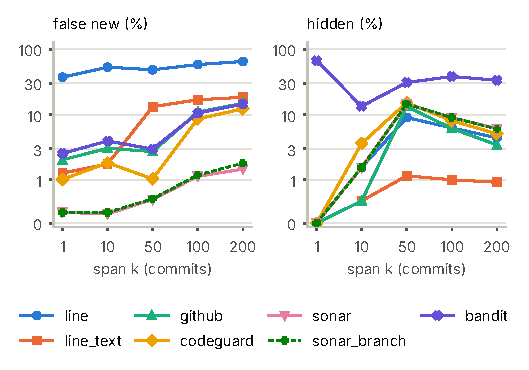
\includegraphics[width=0.9\columnwidth]{fig_drift.pdf}
\caption{Long spans: false-new and hidden rate (percent, symmetric log scale) when a
baseline at an anchor commit is compared with the commit $k$ first-parent steps later.
CodeGuard findings, 105 anchors in 35 repositories, pooled over repositories;
\texttt{drift.csv} has the intervals.}
\label{fig:drift}
\end{figure}

\textit{Semgrep's findings.} On findings from third-party rules
(Table~\ref{tab:rq1-semgrep}) the content schemes keep their false-new order, each paired
difference excluding 0, and Bandit's baseline hides 22.4\% of the new findings.
Semgrep's own ID hides 12.1\% (7.4--18.6), several times more than any other content
scheme, and a gate built on it misses 5.1\% of the 704 commit pairs that introduce a
Semgrep finding. The ID numbers equal matches in file order, so a new match placed
before an equal old one inherits its ID: \texttt{duplicate\_above}
(Section~\ref{sec:rq2}) on real histories. We did not check these findings by hand.

\textit{Long spans.} A baseline is usually compared with code many commits later. From
three anchors per repository, 200, 300 and 400 first-parent commits behind the pin, we
chained the line maps through every commit in between and compared each anchor with the
commit $k$ steps later (Fig.~\ref{fig:drift}). Renames pile up. At $k = 200$, 1,000
renamed files hold 3,813 of the 36,325 persisting findings (10.5\%), and every
path-keyed scheme loses all of them: \texttt{codeguard} reports 12.2\% (1.7--29.6) as
new, \texttt{bandit} 14.5\%, \texttt{github} 14.9\% and \texttt{line\_text} 18.4\%,
against SonarQube's 1.5\% (0.7--2.9). In files that keep their path the gap closes
(\texttt{codeguard} 1.9\%, SonarQube 1.6\%, \texttt{github} 4.9\%). Bandit's baseline
hides about a third of the new findings from $k = 50$ on (33.5\% at $k = 200$). The
other schemes' hidden rates peak at 13--15\% at $k = 50$, with intervals from about 1 to
37\%, and fall to 3--6\% by $k = 200$; a chained line diff has many more steps at which
to lose a line, so we read these as upper bounds.

\section{RQ2: Controlled Changes}\label{sec:rq2}

\begin{figure}[t]
\centering
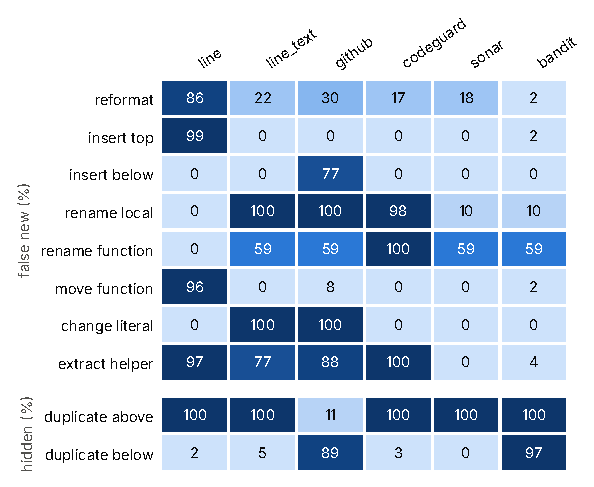
\includegraphics[width=0.9\columnwidth]{fig_rq2.pdf}
\caption{False-new rate for eight transformations, and hidden rate for the two that copy
a finding, in percent, over the 25 Python repositories. \texttt{sonar\_branch} is left
out: no transformation renames a file, so it equals \texttt{sonar} in every cell.}
\label{fig:rq2}
\end{figure}

Fig.~\ref{fig:rq2} reads as a list of blind spots, one or more per scheme.
\texttt{line} fails whenever lines move: 99.1\% after \texttt{insert\_top}, 96.2\% after
\texttt{move\_function}. \texttt{github} fails on a comment inserted \emph{below} the
flagged line (77.5\%), because its hash reads up to 100 characters forward.
\texttt{codeguard} fails when the enclosing scope changes (\texttt{rename\_function} and
\texttt{extract\_helper}, both 100\%) and on renamed locals in the statement (97.9\%),
but masking literals works: after \texttt{change\_literal} it reports none as new, against
100\% for \texttt{line\_text} and 99.6\% for \texttt{github}.

SonarQube comes out best: it reports nothing as new after \texttt{insert\_top},
\texttt{insert\_below}, \texttt{move\_function}, \texttt{change\_literal} and
\texttt{extract\_helper}, since a later pass finds the same line hash elsewhere in the
file, but loses 59.0\% after \texttt{rename\_function}, 17.6\% after \texttt{reformat} and
9.8\% after \texttt{rename\_local}. Renamed functions break the text schemes too (59.5\%
for \texttt{line\_text} and \texttt{github}): 485 of the 822 cases are complexity,
nesting and parameter-count findings on the \texttt{def} line. The \texttt{reformat} row
measures one edit, whose size depends on how the project was formatted before.

The two duplicate rows show what pairing order does. A copy placed above a finding is
paired with the old finding, so the copy is hidden and the original reported as new:
every scheme hides it except \texttt{github} (11.5\%). A copy placed below fools
\texttt{github} instead (88.5\%), since its forward-reading hash moves to the copy, and
\texttt{bandit} hides nearly every copy either way (100\% above, 97.3\% below). After
\texttt{insert\_top}, which moves no code, \texttt{bandit} still reports 2.5\% as new:
three CodeGuard rules put line numbers into their messages (``built on line N'').

\section{Implications}\label{sec:implications}

For tool builders, five changes, in rough order of payoff. Keep the path out of the
identity, or carry identities across renames: here that alone would remove 69\% of
\texttt{codeguard}'s false-new reports. Pair findings one to
one, never by set membership. Fall back on more than one kind of evidence, as SonarQube's
passes do. Mask literals before hashing. Keep locations out of messages that take part
in matching. For users: a gate built on set membership let a third of the commits that
added a Bandit finding through without a report.

\section{Threats to Validity}

\textit{Construct validity.} Our ground truth is a line diff: two findings are the same when they share a rule and the old line maps to the new one, unchanged or edited with a similarity of at least 0.6. A finding whose line is rewritten past that threshold, or moved out of a deleted block, counts as removed plus introduced. We checked 100 findings drawn in five strata from the CodeGuard replays. One author labelled the 60 persisting ones; an LLM rater labelled all 100 without seeing the ground truth or the author's labels; the author then reviewed the 14 findings where the LLM rater said the ground truth was wrong, and agreed on all of them. Re-running the rule showed that three of these, complexity and nesting findings on an unchanged \texttt{def} line, were new after all: the commit had pushed the function over its limit. With the other 11 corrected, the ground truth held for 59 of 60 persisting findings (98.3\%, Wilson 95\% CI 91.1--99.7) and 30 of 40 introduced ones (75.0\%, 59.8--85.8). Every error on an introduced finding was one some scheme had matched to an old finding, so the hidden rates in Table~\ref{tab:rq1} are upper bounds. SonarQube's falls from 1.47\% to an estimated 0.24\% (0.07--0.66), though each corrected rate rests on only 6 to 12 sampled findings. The 27 introduced findings the LLM rater confirmed as new had no human check, and Bandit's own findings were not sampled.

\textit{Internal validity.} We measure ports of each tool's identity method, not the tools. The SonarQube port matched the unmodified Java tracker on 20,000 generated cases, and the Semgrep port reproduced all 716 IDs Semgrep emitted in two replays; the Bandit and GitHub ports agree with \texttt{bandit -b} and with GitHub's \texttt{fingerprints.ts}. SonarQube's branch-mode move detection is modelled only for files git reports as renamed. Some CodeGuard messages contain line numbers, which penalizes methods that compare messages, so we also report Bandit's method on Bandit's own findings, without B101 (91\% of them, nearly all in tests).

\textit{External validity.} The corpus is 35 open-source web applications in Python and JavaScript or TypeScript, each replayed over 200 consecutive commit pairs. Consecutive pairs are the easy case; a real baseline is compared with code many commits later, which we do not measure. A few repositories can dominate a pooled rate, so we report intervals over repositories and per-repository medians. In RQ2 each transformation is applied alone, to one finding, while real commits combine several.


\section{Related Work}\label{sec:related}

\textit{Tracking warnings across versions.} Spacco, Hovemeyer and Pugh treated warning identity as a problem of its own. They added two tracking techniques to FindBugs, so that reviewers could remember warnings already judged safe and see which ones were new, and applied them to Sun's Java runtime library~\cite{spacco2006}. Later work used tracking as a means to another end: Avgustinov et al.\ followed violations through revision histories at Semmle to credit each developer with the violations they introduced or removed~\cite{avgustinov2015}, and Kim and Ernst mined warning histories to rank warning categories by how often fixes removed them~\cite{kim2007}. In both, the tracker is part of the method, and its errors reach the results unmeasured.

The closest work is by Li and Yang~\cite{li2022statictracker}. They labelled the evolution of 3,451 SpotBugs and PMD warnings in four Java projects by hand, showed that an existing tracker failed on refactorings, code shifts and volatile metadata, and proposed StaticTracker, which raised tracking precision from 64.4\% to 90.3\%. Our question is different. We do not build a better tracker; we compare the identity methods that shipped tools use (SonarQube, Bandit, Semgrep and GitHub code scanning), each ported from its source and checked against the tool, on the same findings from 35 Python and JavaScript applications. We also count the two kinds of error separately. A baseline that reports old findings as new is a nuisance; one that hides new findings is a security problem.

\textit{Why identity matters in practice.} Developers name false positives and the way warnings are presented as barriers to using static analysis~\cite{johnson2013}, and at Google, the analyses developers act on show their findings in code review, before the code is committed~\cite{sadowski2015tricorder,sadowski2018lessons}. Showing a developer only the findings their change introduced needs exactly the identity we measure. Suppressions depend on it too: Hu et al.\ found that half of the suppression comments in their study suppress no warning at all~\cite{hu2025suppressed}. SARIF~2.1.0 gives tools fields for fingerprints and for a result's baseline state~\cite{sarif2020}, yet the tools we compare match results in very different ways (Section~\ref{sec:schemes}).


\section{Conclusion}\label{sec:conclusion}

Most of the losses of shipped tools' content-based methods come from one design choice,
the file path inside the identity, and the costliest error, hiding a new finding, comes
mostly from another, matching by set membership. Neither needs a better analyzer to fix.
Long-lived baselines make the first choice costlier: 200 commits after an anchor, a
tenth of the persisting findings sit in renamed files.

\textit{Data availability.} The replay tool, the ports and their checks, the corpus with
its pinned commits, the results, the ground-truth sample with both raters' labels, and
the scripts that produce every table and figure are
\ifanon
available to reviewers through the venue's anonymous artifact channel, licensed
Apache-2.0.
\else
at \url{https://github.com/mevichitra/codeguard} under
\texttt{research/finding\_identity/}, licensed Apache-2.0.
\fi

\bibliographystyle{IEEEtran}
\bibliography{references}

\end{document}
